\documentclass[11pt,letterpaper]{article}
\usepackage[top=2.0cm, bottom=3cm, left=2.0cm, right=2.0cm]{geometry}
\usepackage[utf8]{inputenc}
\usepackage[T1]{fontenc}
\usepackage[spanish]{varioref}
\usepackage[activeacute, spanish, es-tabla]{babel}
\usepackage{fancyhdr}
\usepackage{multicol}
\usepackage{float}
\usepackage{textcomp}
\usepackage{ae,aecompl}
\usepackage{amssymb,amsmath}
\usepackage[pdftex]{graphicx}
\pagestyle{fancy} 
\pagenumbering{arabic} 
\renewcommand{\headrulewidth}{0pt} 
\setlength{\headsep}{20pt} 
\setlength{\headheight}{65pt} 
\setlength{\textheight}{600pt} 
\setlength{\columnsep}{15pt} 
\newcommand{\universidad}{\small{Universidad Técnica Federico Santa María}}
\newcommand{\campus}{\small{Campus Santiago San Joaquín}}
\newcommand{\semestre}{\small{Segundo Semestre 2016}}

% Definiciones de Título e Integrantes de Experiencia
\newcommand{\titulo}{Tarea 2 - TALF}
\newcommand{\integrantes}{\begin{tabular}{c}
Jorge Contreras 201573547-6 \\
Juan Pablo Jorquera  201573533-6 \\
\end{tabular}}

\renewcommand{\maketitle}
{
\thispagestyle{fancy}
\begin{center}
\begin{Large}
\textbf{\titulo}\\
\end{Large}
\vspace{0.5cm}
\integrantes
\end{center}
\vspace{0.3cm}
}


%ENCABEZADO

\fancyhead[R]{\begin{minipage}[b]{0.405\textwidth}
\begin{center}
\universidad \\ 
\campus \\ 
\lab \\ 
\semestre
\end{center}
\end{minipage}}
\fancyhead[L]{\vspace{15pt}
\includegraphics[height=1.6cm]{Escudo.png}}
%%%%%%%%%%%%%%%%%%%%%%%%%%%%%%%%%%%%%%%%%%%%%%%%
%                                              %
% AQUI TERMINAN LAS DEFINICIONES DE ENCABEZADO %
% Y EMPIEZA EL CUERPO DEL DOCUMENTO            %
%                                              %
%%%%%%%%%%%%%%%%%%%%%%%%%%%%%%%%%%%%%%%%%%%%%%%%

\begin{document}
\maketitle

\section{Pregunta 1}
Primero realizamos el AFD de la tabla para poder trabajar sobre él.

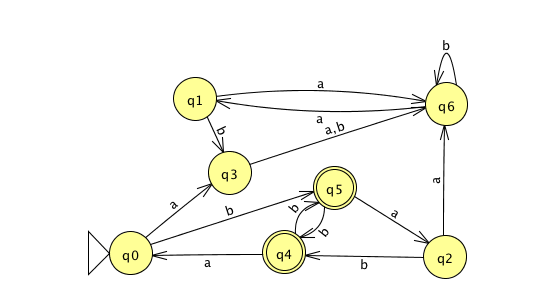
\includegraphics[height=5cm]{tarea_1.png}
\subsection{Parte (a)}
Primero hacemos la tabla correspondiente al autómata.

\begin{table}[h]
\centering
\label{tabla_min}
\begin{tabular}{lllllll}
q1 & X  &    &    &    &    &    \\
q2 & O  & X  &    &    &    &    \\
q3 & X  & O  & X  &    &    &    \\
q4 & X  & X  & X  & X  &    &    \\
q5 & X  & X  & X  & X  & O  &    \\
q6 & X  & O  & X  & O  & X  & X  \\
   & q0 & q1 & q2 & q3 & q4 & q5
\end{tabular}
\caption{Tabla de equivalencias}
\end{table}

Luego continuamos eliminando los que son equivalentes:
\newpage
\begin{itemize}
\item{Eliminar q2:}

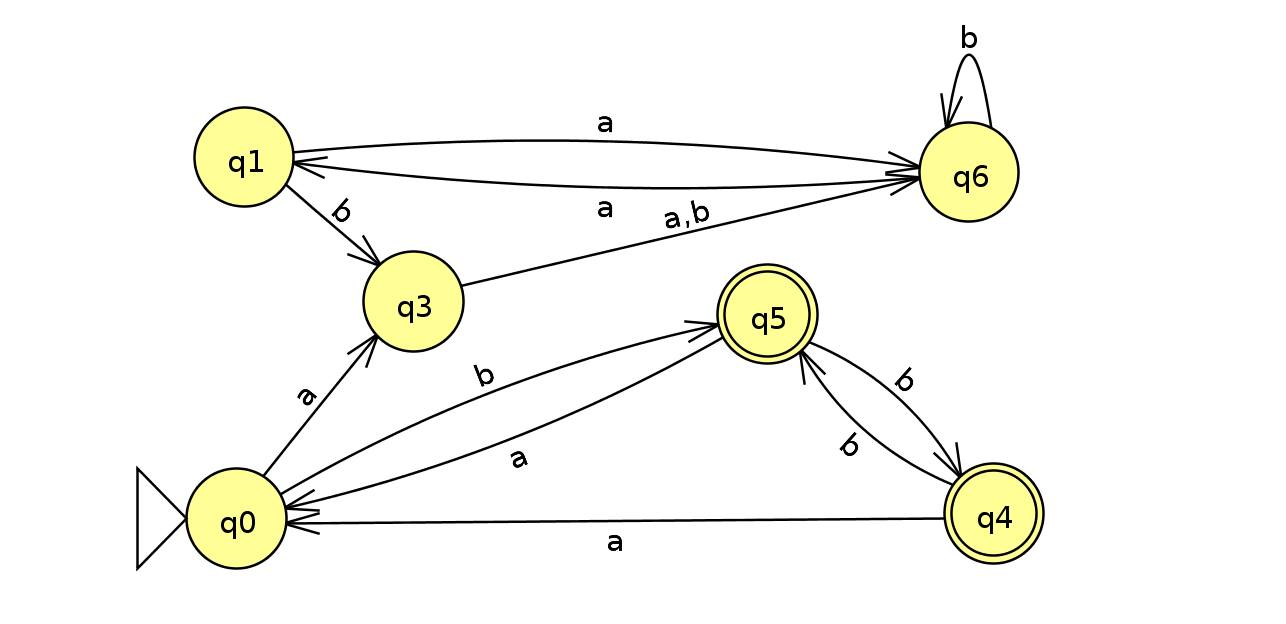
\includegraphics[height=5cm]{tarea_1-a.png}

\item{Eliminar q5:}

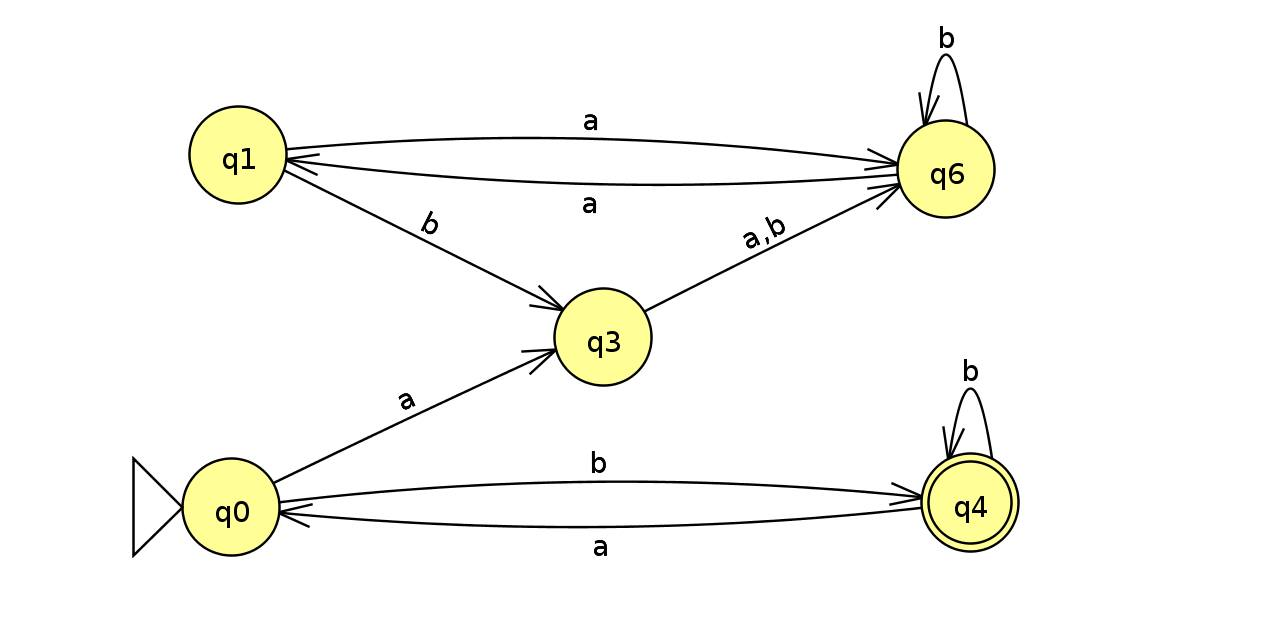
\includegraphics[height=5cm]{tarea_1-a-2.png}

\item{Eliminar q3:}

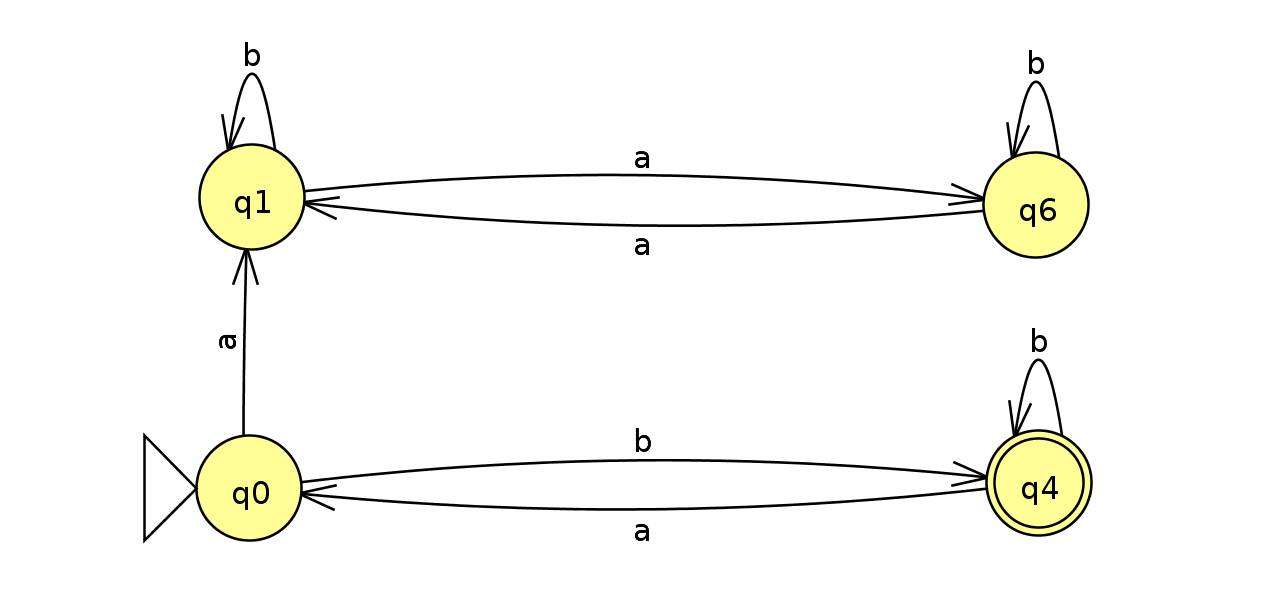
\includegraphics[height=5cm]{tarea_1-a-3.png}
\newpage
\item{Eliminar q6:}

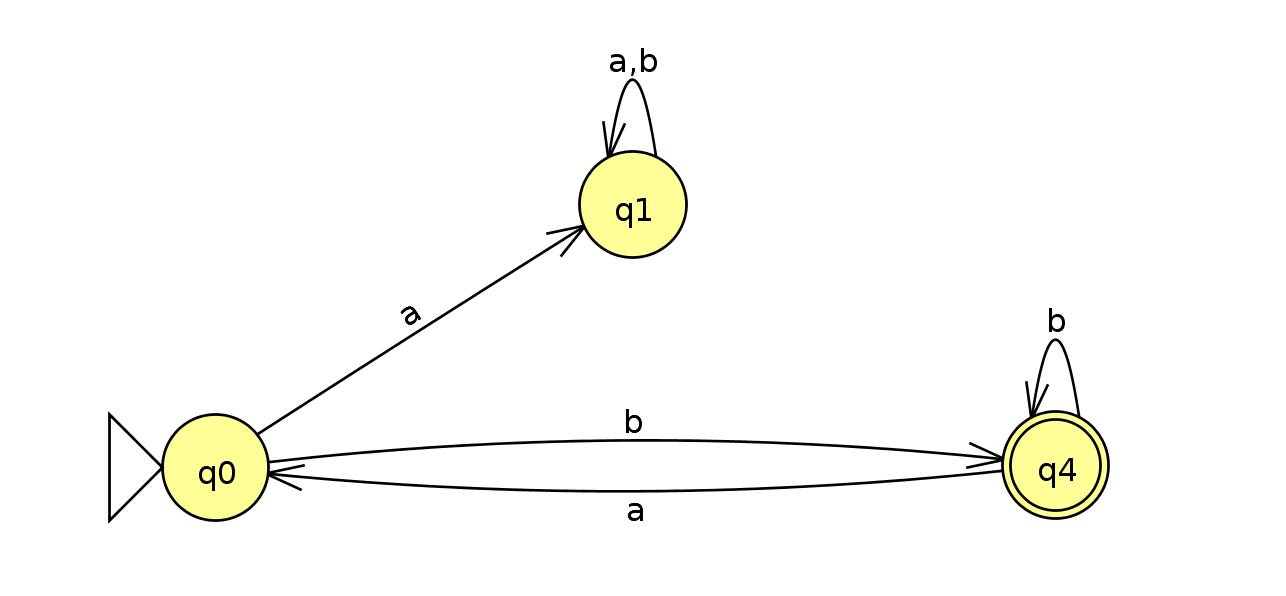
\includegraphics[height=5cm]{tarea_1-a-4.png}
\end{itemize}


\subsection{Parte (b)}
\begin{itemize}
	\item{Tomando q0 y q1: la palabra ``b'' distingue a ambos, ya que quedan en distinto estado de aceptación.}
	\item{Tomando q0 y q4: simplemente ``ab'' los distingue.}
	\item{Tomando q1 y q4: ``b'' los distingue.}
\end{itemize}

\subsection{Parte (c)}
\begin{itemize}
\item{Primero normalizamos para tener un nodo de entrada y de salida claros.}
\begin{center}
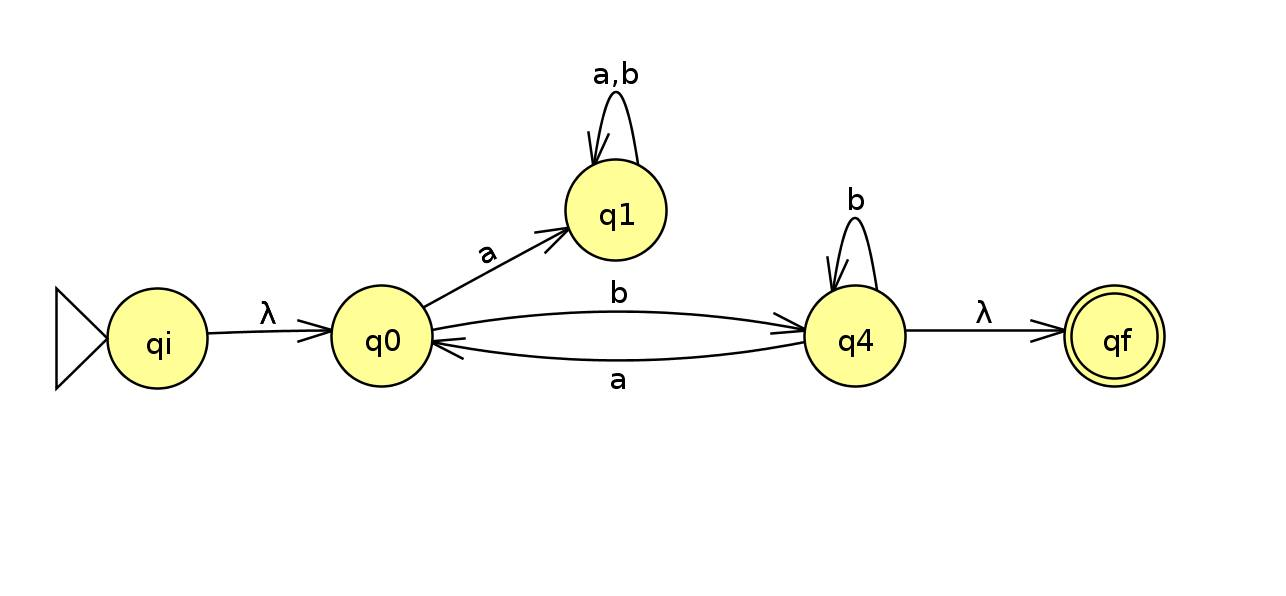
\includegraphics[height=4.3cm]{tarea_1-c.png}
\end{center}
\item{Luego eliminamos el nodo ``basura'' que se encuentra.}
\begin{center}
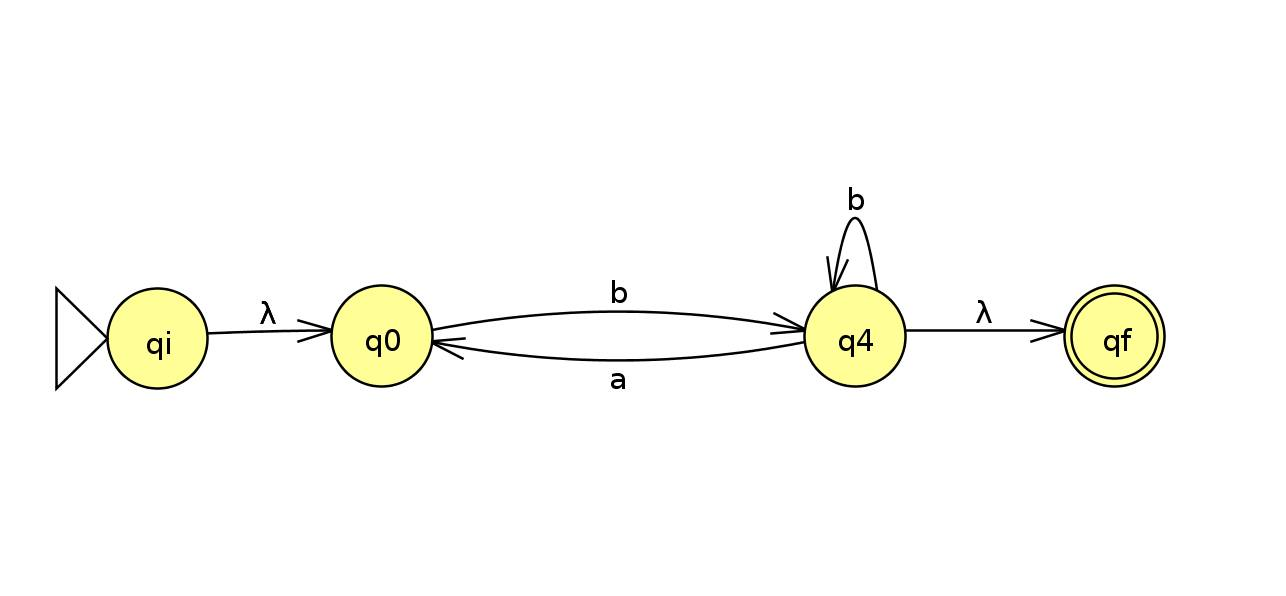
\includegraphics[height=4.3cm]{tarea_1-c2.png}
\end{center}
\item{Eliminamos q4.}
\begin{center}
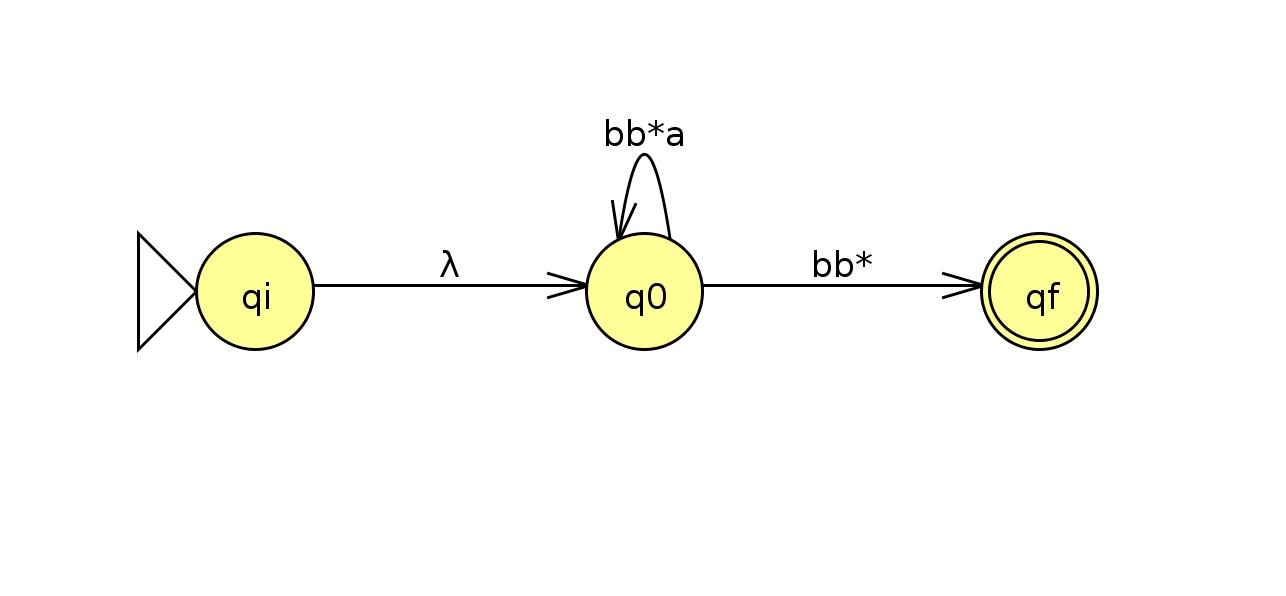
\includegraphics[height=4.3cm]{tarea_1-c3.png}
\end{center}
\item{Finalmente eliminamos q0.}
\begin{center}
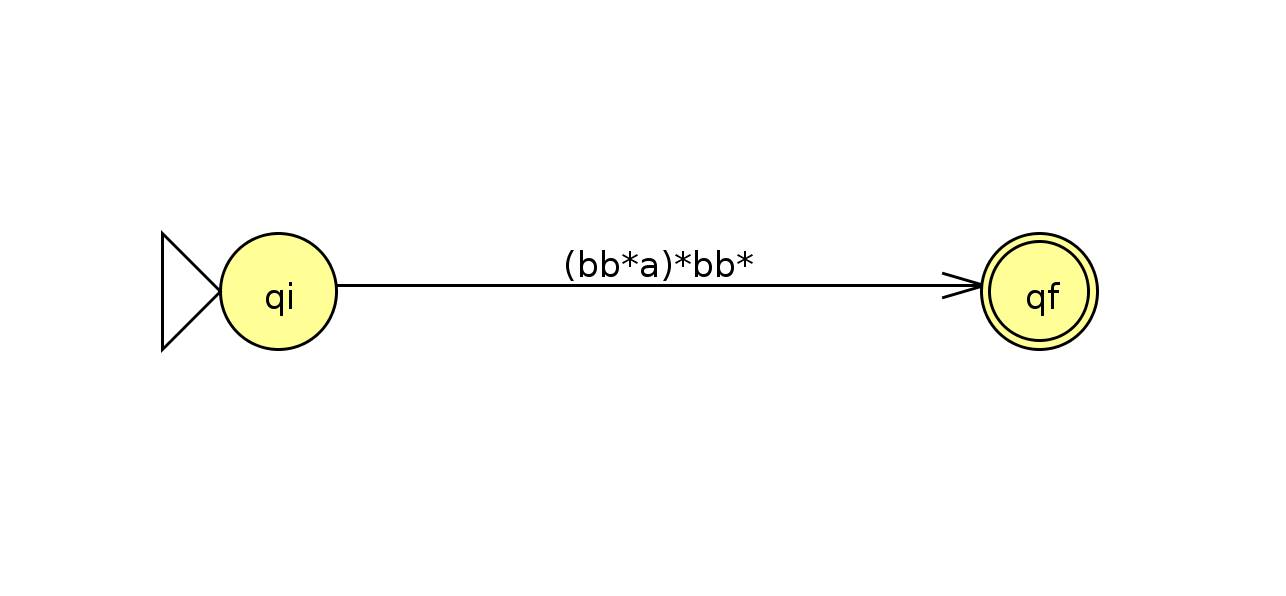
\includegraphics[height=4.3cm]{tarea1-c4.png}
\end{center}
\end{itemize}

\subsection{Parte (d)}
Corresponde al lenguaje que comienza con una o más ``b'' y, si lo sigue una ``a'', se repite el proceso con ``b'' nuevamente.

\section{Pregunta 2}
Si tomamos $L_B = LL_bL$ \hspace{0.1cm} donde $L_b = \{b\}$, claramente $L_B$ y $L_b$ son regulares al ser parte L. Por otro lado tenemos que: 
\begin{equation}
	L' \Leftrightarrow L_B - L_b
\end{equation}

Usando propiedades de conjuntos tenemos:
\begin{equation}
	L' \Leftrightarrow L_B - L_b \Leftrightarrow  L_B \cap L_b^c
\end{equation}
Donde por propiedades de clausura se sabe que como $L_b$ es regular, entonces $L_b^c$ también es regular. De igual forma, se deduce que la intersección de ambos lenguajes regulares $L_B$ y $L_b^c$ es regular, por lo que $L'$ también es regular.


\section{Pregunta 3}
\subsection{Parte (a)}
Sea $w = a^nb^{n-1}$, $w \in  L_{1}$

$w = xyz$, con $|xy| \leqslant n$ ; $|y|\geqslant 1$.
 \\

Necesariamente x e y están dentro de $a^n$, Así:

$x = a^p$, $p \geqslant 0$

$y = a^q$, $q\geqslant 1$

$z = a^{n-p-q}b^{n-1}$
 \\

Aplicamos Teorema del Bombeo, k veces y.
 \\
 
$xy^kz = a^{n+q(k-1)}b^{n-1}$
 \\

Para que la palabra pertenezca a $L_{1}$ se debe cumplir que:
 \\
 
$|n+q(k-1) - (n-1)| \leqslant 42$

$|q(k-1) -1| \leqslant 42$
 \\
 
Elegimos k=50, quedando

$|49q - 1| \leqslant 42$

Como $q \geqslant 1$, lo anterior es una contradicción y por lo tanto el lenguaje $L_{1}$ No es regular.


\subsection{Parte (b)}
Sea $w = a^nca^n, w \in  L_{2}$

$w = xyz$, con $|xy| \leqslant n ; |y| \geqslant 1$
 \\

Necesariamente x e y están dentro de $a^n$, Así:

$x = a^p$, $p \geqslant 0$

$y = a^q$, $q \geqslant 1$

$z = a^{n-p-q}ca^n$
 \\

Aplicamos Teorema del Bombeo, k veces y.
 \\
 
$xy^kz = a^{n+q(k-1)}ca^n$
 \\

Para que la palabra pertenezca a $L_{2}$ se debe cumplir que:
 \\
 
$n+q(k-1) = n$

$q(k-1) = 0$
 \\
 
Elegimos k=2, quedando

q = 0

Pero $q \geqslant 1$, por lo cual la palabra no pertenece al lenguaje y así demostramos que $L_{2}$ No es regular.

\subsection{Parte (c)}
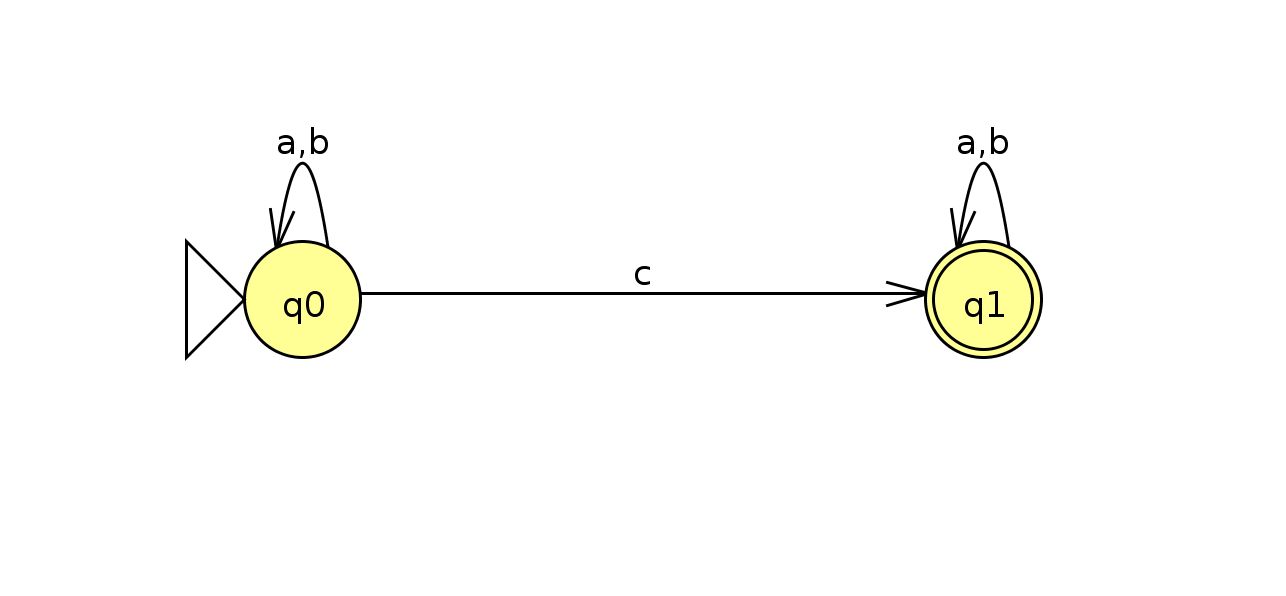
\includegraphics[height=5cm]{tarea_3-c.png}

Como pudimos generar un autómata para el lenguaje, éste es regular.


\subsection{Parte (d)}
Sea $w = a^{2n}b^{2n-1}$, $w \in  L_{4}$

$w = xyz$, con $|xy| \leqslant 2n$ ; $|y| \geqslant 1$.
 \\

Necesariamente x e y están dentro de $a^{2n}$, Así:

$x = a^p$, $p \geqslant 0$

$y = a^q$, $q \geqslant 1$

$z = a^{2n-p-q}b^{2n-1}$
 \\

Aplicamos Teorema del Bombeo, k veces y.
 \\
 
$xy^kz = a^{2n+q(k-1)}b^{2n-1}$
 \\

Para que la palabra pertenezca a $L_{4}$ se debe cumplir:
 \\
 
(1)

$2n+q(k-1) > 2n-1$

$q(k-1) > -1$
 \\
 
Elegimos k=0, quedando

$-q > -1$

$q < 1$

Pero $q \geqslant 1$, existiendo así una contradicción.
 \\
 
(2) 

$2n+q(k-1)$ es par
 \\
 
Elegimos $k = \frac{1}{q} + 1$

$2n+q(\frac{1}{q} + 1 -1)$

$2n+1$

Lo cual siempre es impar.
 \\

Como no se cumple ni (1) ni (2), podemos asegurar que el lenguaje L$_{4}$ No es regular


\subsection{Parte (e)}
El metro de Santiago posee 5 líneas y 100 estaciones en total, pudiendo llegar desde cualquier estación de cualquier línea a otra estación de cualquier línea igualmente, es decir, es un grafo conexo. Como la cantidad de estaciones es finita, se puede crear un automáta finito en el cual las estaciones hacen de estados, y las transiciones de los estados corresponden a las estaciones que se encuentran inmediatante conectadas a otra estación, por ejemplo Camino Agrícola posee dos transiciones, a San Joaquín y a Carlos Valdovinos, mientras que Los Heroes posee 4 transiciones, a Toesca, Santa Ana, Moneda y República. Cada transición entre estados está ligada a la primera letra del nombre del estado al cual se llega, habiendo un estado inicial qo(que no corresponde a ninguna estación de metro) que llega a todos los demás estados(estaciones) usando las transiciones explicadas anteriormente, y todos los estados del autómata finito son estados de aceptación. A continuación se presenta un modelo reducido del automáta que abarca sólo a la estación Baquedano y sus respectivas transiciones(considerando que el automáta total es demasiado denso).
 \\
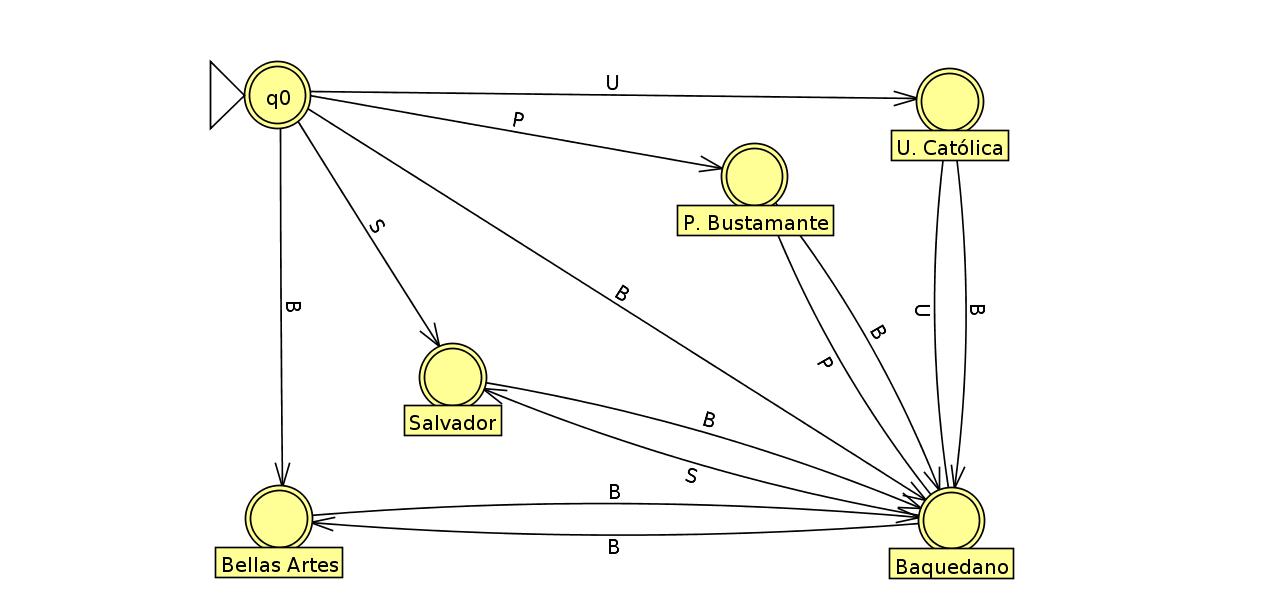
\includegraphics[height=5cm]{tarea_3-e.png}
 \\
Como es posible la creación de un autómata finito, el lenguaje L$_{5}$ es regular.


\section{Pregunta 4}
\subsection{Parte (a)}
Como se puede ver el AFND a continuación, antes del $n-$ésimo símbolo (contado desde atrás) no importa lo que haya, por lo que se produce un loop, luego continua con dicho símbolo seguido por $n-$estados, por lo que en éste autómata hay $n+1$ estados.

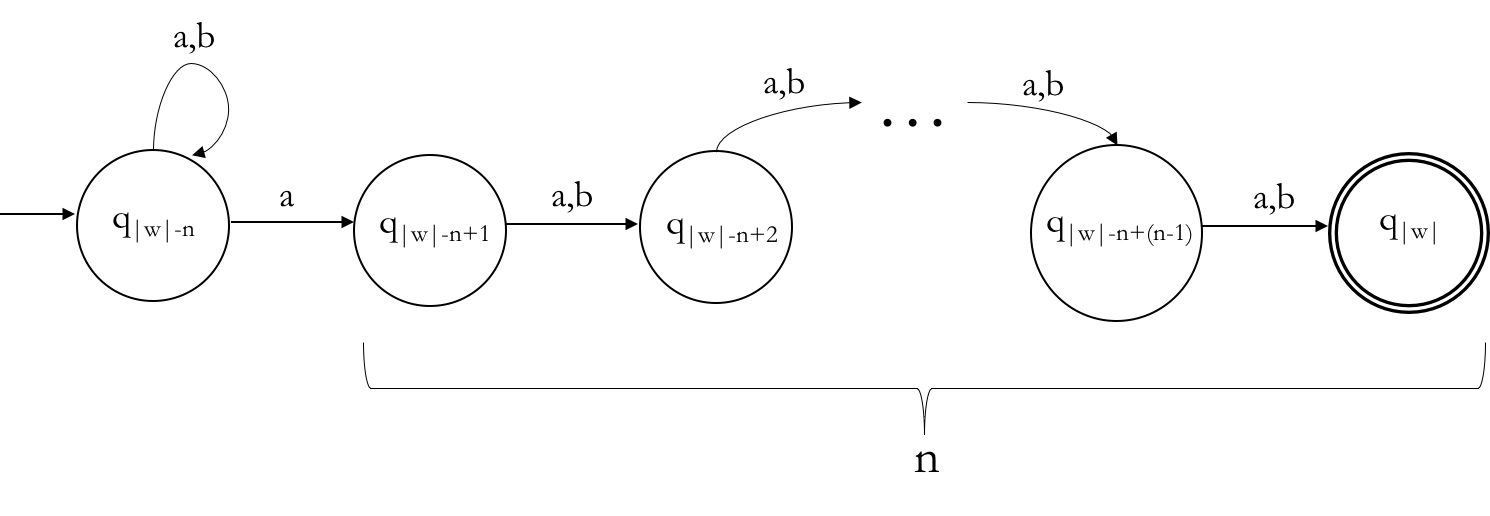
\includegraphics[height=5cm]{tarea_4-a.png}
\subsection{Parte (b)}
En primer lugar damos más importancia para cada estado después de la ``a'' requerida (inicialmente siempre hay un loop de ``b'', ya que no importa lo que esté concatenado antes), encontes verificamos lo que podemos concatenar después según Myhill-Nerode, ya que dependiendo del $n$ puede variar el resultado, por ejemplo si tenemos (a partir del $n$-ésimo caracter):
\begin{itemize}
\item{``aa'': Al concatenar al final de la palabra ``a'' se distingue convirtiéndose el segundo ``a'' en el nuevo $n$-ésimo y quedando finalmente en aceptación.}
\item{``ab'': Por otro lado si concatenamos ``a'' en este caso el ``b'' pasaría a ser el $n$-ésimo quedando fuera de la aceptación.}
\end{itemize}
Entonces nos damos cuenta que para cada caracter después del $n$-ésimo caracter se crean clases de equivalencia distintas diferenciándose en cual es la última posición de ``a'' y pudiéndo volver a éstas según corresponda, por lo que es necesario crear dos estados nuevos por cada caracter de $n$, por lo que finalmente la cantidad de estados será por lo menos $2^n$. Cabe resaltar que la mitad de $2^n$ serán de aceptación al estar en el último nivel y que en uno de ellos se encontrará un loop de ``a'', ya que si se sigue un camino de sólo ``a'' da lo mismo las que se agreguen, el $n$-ésimo seguirá siendo ``a''. \\

A continuación se muestra un ejemplo para $n = 2$, para ayudar la visualización.

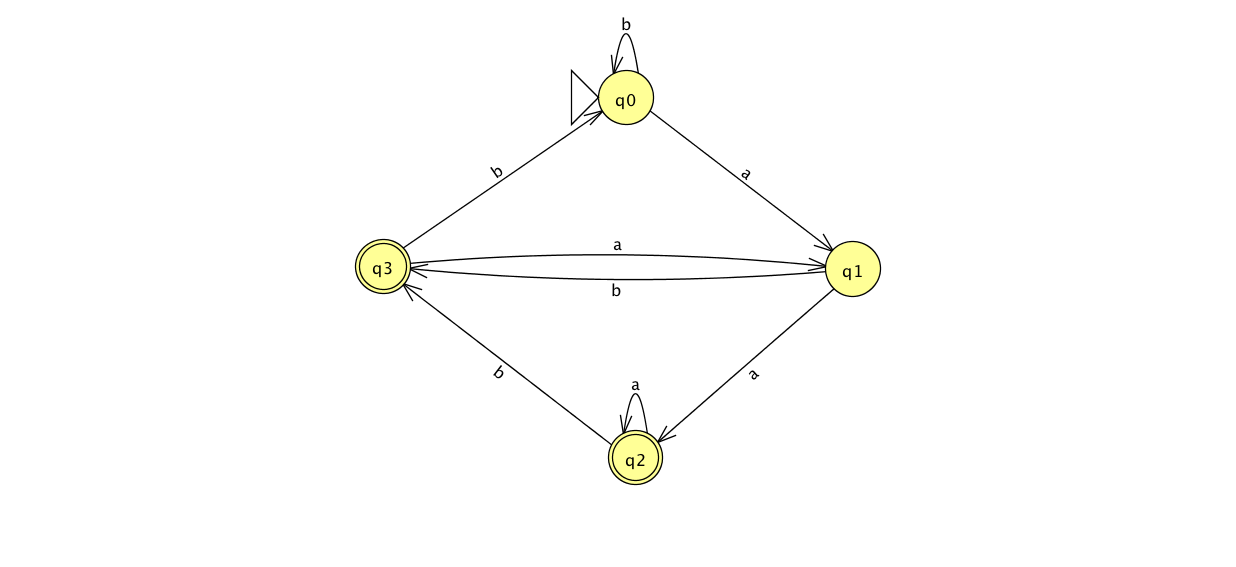
\includegraphics[height=10cm]{tarea_4-b.png}


\section{Pregunta 5}
\subsection{Parte (a)}
Es decidible, ya que dado un lenguaje regular, con su respectivo AFD (o AFND), siempre se puede identificar si alguna de las palabras que aceptan es. Una forma de realizar esto sería:

\begin{enumerate}
	\item Ver caminos posibles desde el inicio hasta cualquier estado de aceptación.
	\item Calcular distancia de dichos caminos ignorando los loops que se encuentren, si ésta es de tamaño par, inmediatamente se cumple. Por otro lado si es de tamaño impar, hay que verificar loops que se encuentren:
	\begin{itemize}
		\item Si hay un loop de tamaño par, simplemente ignorar, ya que no afecta la paridad de la palabra.
		\item Si, por otro lado, hay loop de tamaño impar (incluyen los que se hacen sobre el mismo estado), se cumple la condición, ya que se puede recorrer cualquier número de veces el loop hasta formar la paridad requerida.
		\item Si simplemente no hay loops o si todos ellos eran de tamaño par, significa que el lenguaje no cumple con incluir palabras de largo par.
	\end{itemize}
\end{enumerate}

\subsection{Parte (b)}
En este caso, el problema también es decidible, una forma de hacer eso es tomando el algoritmo usado en la Parte (a) y modificarlo en el punto 1:
La única diferencia es que en vez de realizar el proceso para cualquier camino entre el inicio y estado de aceptación, se debe hacer para todo camino posible hacia todo estado de aceptación, para así verificar la paridad para la totalidad del lenguaje.

\subsection{Parte (c)}
También resulta un problema decidible, para ello tomamos el AFD mínimo del lenguaje que se requiera identificar y sobre él verificamos si ya es par, en caso de no ser:
\begin{itemize}
	\item Tomar un estado que tenga más de un camino entrante. Si hay, se puede agregar un estado adicional:
		\begin{enumerate}
			\item Dirigir alguno de los caminos entrantes hacia un nuevo estado, que cumpla la misma aceptación que el objetivo anterior.
			\item Copiar caminos que partan del estado anterior, esta ver partiendo desde el estado nuevo.
			\item Finalmente con dicho estado, el AFD tiene una cantidad par de estados.
		\end{enumerate}
	\item En caso de no haber, no se pueden agregar más estados y no hay ADF con cantidad par de estados.
\end{itemize}

Un ejemplo de un caso en que no haya AFD con cantidad par de estados se muestra a continuación com un alfabeto = \{a\}:
\begin{center}
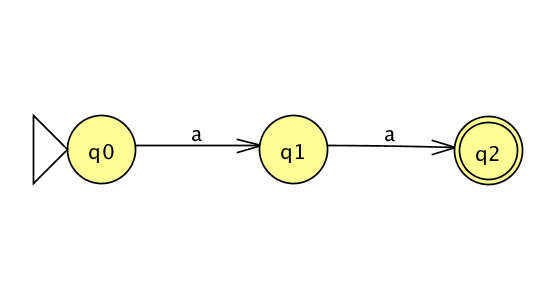
\includegraphics[height=6cm]{tarea_5-c.png}
\end{center}

Se ve que no se pueden agregar estados adicionales, ya que para agregar alguno sobre los caminos que llegan a q1 o q2, habría simplemente que reemplazar el estado elegido, dejándolo inalcanzable y sacándolo así del AFD.

El caso opuesto lo vemos con el siguiente AFD que cumple la condición:
\begin{center}
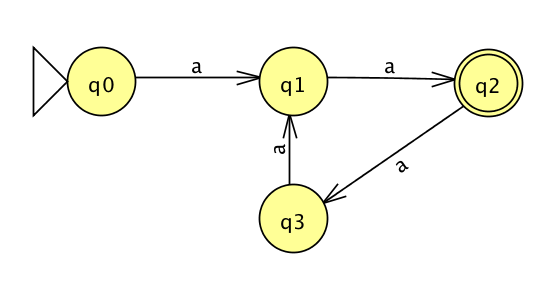
\includegraphics[height=5cm]{tarea_5-c2.png}
\end{center}

Donde obligatoriamente de elige q1 y se puede agregar un estado sobre cualquiera de los dos caminos, un ejemplo de ello sería:
\begin{center}
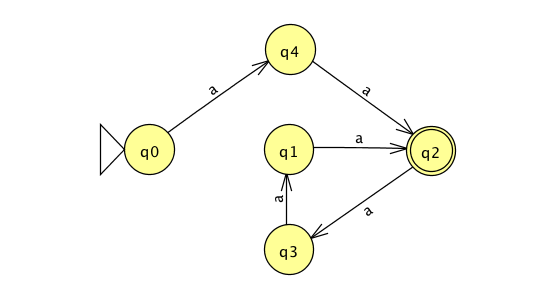
\includegraphics[height=6cm]{tarea_5-c3.png}
\end{center}

Donde se utilizan los pasos mencionados y se deja
el AFD inalterado para el lenguaje que lo representa, esta vez con una cantidad par de estados

\end{document}
